\subsection{Théorème de CAP: }
Le théorème de CAP est l’acronyme de « Coherence », « Availability » et « Partition tolerance », aussi connu sous le nom de théorème de Brewer. Ce théorème, formulé par Eric Brewer en 2000 et démontré par Seth Gilbert et Nancy Lych en 20025, énonce une conjecture qui définit qu’il est impossible, sur un système informatique de calcul distribué, de garantir en même temps les trois contraintes suivantes :

\begin{itemize}[label=\textbullet]
\item \textbf{« Coherence » (Cohérence) :} Tous les clients du système voient les mêmes données au même instant.
\item \textbf{« Availibility » (Haute disponibilité) :} Un système est dit disponible si toute requête reçue par un noeud retourne un résultat. Bien évidemment le noeud en question ne doit en aucun cas être victime de défaillance.
\item \textbf{« Partition tolerance » (Tolérance à la partition) :} Un système est dit tolérant à la partition s’il continue à répondre aux requêtes de manière correcte même en cas de panne autre qu’une panne totale du système.
\end{itemize}

\begin{figure}[h]
	\centering
    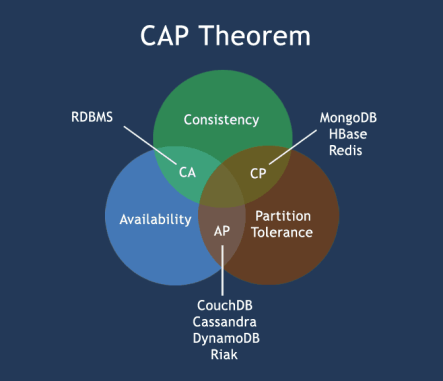
\includegraphics[scale=0.5]{img/4.1}
    \caption{Théorème de CAP}
\end{figure}

Seules deux des trois contraintes peuvent être respectées en même temps. Un des premiers buts des systèmes NoSQL est de renforcer la « scalabilité » horizontale, il faut pour cela que le principe de tolérance au partitionnement soit respecté, ce qui exige l’abandon soit de la cohérence, soit de la haute disponibilité.

\subsubsection{Haute disponibilité et tolérance à la partition: (AP)}
Les bases ne sont pas forcément cohérentes dans le temps mais la multiplicité des bases sur le réseau permet de garantir une réponse quoi qu'il arrive.

En effet, cela voudrait dire que les utilisateurs n’ont pas forcément tous la même vue à un moment donné. Dans certains cas cela peut poser des problèmes, mais bien souvent ce n’est pas une nécessité. Prenons l’exemple de deux utilisateurs qui sont amis sur Facebook, Marcel et Pierre. Si Marcel partage une photo sur son « mur » et que Pierre au même instant ne la voit pas dans son « fil d’actualité » elle apparaîtra dans les prochaines secondes. Dans ce cas précis, est-ce un problème pour Pierre d’attendre environ une minute pour voir la photo que vient de publier son ami Marcel ?

\subsubsection{Cohérence et tolérance à la partition: (CP)}
Un tel système de base de données stocke les données dans les nœuds distribués, mais assure également la cohérence de ces données, mais le support n'est pas assez bon pour la disponibilité.

La plupart du temps, les systèmes NoSQL qui garantissent une forte cohérence des données sont architecturés en maître/esclave. Cela veut dire que toutes les écritures doivent être faites sur le serveur maître, et en cas de panne de ce dernier, les opérations d’écriture, de modification et de suppression ne deviennent plus disponibles. Seule la lecture des données sur les serveurs esclaves est possible.

\subsubsection{Cohérence et Haute disponibilité (CA):}
Tous les clients du système voient les mêmes données au même instant. Notamment les deux propriétés respectées par les bases de données relationnelles. 

